\documentclass[article,nojss]{jss}\usepackage[]{graphicx}\usepackage[]{color}
% maxwidth is the original width if it is less than linewidth
% otherwise use linewidth (to make sure the graphics do not exceed the margin)
\makeatletter
\def\maxwidth{ %
  \ifdim\Gin@nat@width>\linewidth
    \linewidth
  \else
    \Gin@nat@width
  \fi
}
\makeatother

\definecolor{fgcolor}{rgb}{0.345, 0.345, 0.345}
\newcommand{\hlnum}[1]{\textcolor[rgb]{0.686,0.059,0.569}{#1}}%
\newcommand{\hlstr}[1]{\textcolor[rgb]{0.192,0.494,0.8}{#1}}%
\newcommand{\hlcom}[1]{\textcolor[rgb]{0.678,0.584,0.686}{\textit{#1}}}%
\newcommand{\hlopt}[1]{\textcolor[rgb]{0,0,0}{#1}}%
\newcommand{\hlstd}[1]{\textcolor[rgb]{0.345,0.345,0.345}{#1}}%
\newcommand{\hlkwa}[1]{\textcolor[rgb]{0.161,0.373,0.58}{\textbf{#1}}}%
\newcommand{\hlkwb}[1]{\textcolor[rgb]{0.69,0.353,0.396}{#1}}%
\newcommand{\hlkwc}[1]{\textcolor[rgb]{0.333,0.667,0.333}{#1}}%
\newcommand{\hlkwd}[1]{\textcolor[rgb]{0.737,0.353,0.396}{\textbf{#1}}}%
\let\hlipl\hlkwb

\usepackage{framed}
\makeatletter
\newenvironment{kframe}{%
 \def\at@end@of@kframe{}%
 \ifinner\ifhmode%
  \def\at@end@of@kframe{\end{minipage}}%
  \begin{minipage}{\columnwidth}%
 \fi\fi%
 \def\FrameCommand##1{\hskip\@totalleftmargin \hskip-\fboxsep
 \colorbox{shadecolor}{##1}\hskip-\fboxsep
     % There is no \\@totalrightmargin, so:
     \hskip-\linewidth \hskip-\@totalleftmargin \hskip\columnwidth}%
 \MakeFramed {\advance\hsize-\width
   \@totalleftmargin\z@ \linewidth\hsize
   \@setminipage}}%
 {\par\unskip\endMakeFramed%
 \at@end@of@kframe}
\makeatother

\definecolor{shadecolor}{rgb}{.97, .97, .97}
\definecolor{messagecolor}{rgb}{0, 0, 0}
\definecolor{warningcolor}{rgb}{1, 0, 1}
\definecolor{errorcolor}{rgb}{1, 0, 0}
\newenvironment{knitrout}{}{} % an empty environment to be redefined in TeX

\usepackage{alltt}



\usepackage{float}
\usepackage{framed}
\usepackage{subcaption}
\usepackage{amsmath}
\usepackage[ruled,vlined]{algorithm2e}
\usepackage{listings}
\usepackage[shortcuts]{extdash}
\renewcommand{\subfloat}[2][need a sub-caption]{ \subcaptionbox{#1}{#2} }


%\addbibresource{paper2.bib}
\def\cov{{\text{COV}}}
\def\E{{\text{E}}}
\def\T{{\footnotesize{^{_{\sf T}}}}}
\setkeys{Gin}{width=0.45\textwidth}
\setcitestyle{square}




\newcommand{\class}[1]{`\code{#1}'}
\newcommand{\fct}[1]{\code{#1()}}



\author{Ruoyong Xu\\University of Toronto
   \And Patrick Brown\\University of Toronto}
\Plainauthor{Ruoyong Xu, Patrick Brown}


\title{Random number generation and applications on GPU’s in R?}
\Plaintitle{}
\Shorttitle{}


\Abstract{
Parallel processing by graphics processing unit (GPU) can be used to speed up computationally intensive tasks, which when combined with \proglang{R}, it can largely improve \proglang{R}’s downsides in terms of slow speed, memory usage and computation mode.  There is currently no \proglang{R} package that does random number generation on GPU, while random number generation is critical in simulation-based statistical inference and modeling. We introduce the \proglang{R} package \pkg{gpuRandom} that leverages the \pkg{gpuR} package, and can generate random numbers on GPU by utilizing the \pkg{clRNG} (OpenCL) library, the package enables reproducible research by setting random streams on GPU and can thus accelerate several types of simulation and modelling.  \pkg{gpuRandom} is portable and flexible, developers can use its random number generation kernel for various other purposes and applications. 
}


\Keywords{GPU, \pkg{gpuRandom} package, parallel computing, \pkg{clRNG} library}
\Plainkeywords{GPU, gpuRandom package, parallel computing, clRNG library}


\Address{
  Ruoyong Xu\\
  Department of Statistics\\
  University of Toronto\\
  Universit\"at Innsbruck\\
  Universit\"atsstr.~15\\
  6020 Innsbruck, Austria\\
  E-mail: \email{ruoyong.xu@mail.utoronto.ca}}


\Address{
  Achim Zeileis\\
  Journal of Statistical Software\\
  \emph{and}\\
  Department of Statistics\\
  University of Toronto\\
  Universit\"at Innsbruck\\
  Universit\"atsstr.~15\\
  6020 Innsbruck, Austria\\
  E-mail: \email{ruoyong.xu@mail.utoronto.ca}}
\IfFileExists{upquote.sty}{\usepackage{upquote}}{}
\begin{document}
%\SweaveOpts{concordance=FALSE}




\section[Introduction]{Introduction}

\begin{leftbar}
% Why?
% 
% gpu massively parallel and relatively cheap, useful for stats
% there are gpu packages in R, gpuR
% no random numbers yet.  complicated to do on gpu, need multiple seeds becuase of parallel generation
% reproducability: need to save current state and restore

In recent years, parallel computing with R \citep{r2021} has become a very important topic and attracted lots of interest from researchers \citep[see][for a review]{eddelbuettel2021parallel}. Although \proglang{R} is one of the most popular statistical software with many advantages, it has drawbacks in memory usage and computation mode aspects \citep{zhao_2016}. To be more specific, (1) \proglang{R} requires all data to be loaded into the main memory (RAM) and thus can handle a very limited size of data; (2) \proglang{R} is a single-threaded program, it can not effectively use all the computing cores of multi-core processors. Parallel computing is the solution to these drawbacks of \proglang{R}, for an overview of current parallel computing approaches with \proglang{R}, see CRAN Task View by \citet{cran2021} at \url{https://cran.r-project.org/web/views/HighPerformanceComputing.html}. One major way of parallel computing with \proglang{R} is using Graphics Processing Units (GPUs). GPUs can perform thousands of tests simultaneously, which makes them powerful at doing massive parallel computing and they are relatively cheap compared to multicore CPU's. Although there has been a few \proglang{R} packages developed that provide some GPU capability in the past years, they come with some restrictions. Packages such as \pkg{gputools}, \pkg{gpumatrix}, \pkg{cudaBayesreg}, \pkg{rpud} (available on github), are now no longer maintained, the popular \pkg{tensorflow} \citep{tensorflow1} package uses GPU via \proglang{Python}, which makes it hard to be incorporated in a new \proglang{R} package that uses GPU. All of these mentioned packages are restricted to \proglang{R} users with NVIDIA GPUs. \pkg{gpuR} \citep{gpur1} is the only \proglang{R} package with a convenient interface between \proglang{R} and GPUs and it is created for any \proglang{R} user with a GPU device. By utilizing the \pkg{ViennaCL} \citep*{rupp2016viennacl} library, it provides a bridge between \proglang{R} and non-proprietary GPUs through an \proglang{OpenCL} (Open Computing Language) backend, which when combined with \pkg{Rcpp} \citep{rcpp1} gives a building block for other \proglang{R} packages. 

Random number generator (RNG) is critical in simulation-based statistical inference, there is not yet an \proglang{R} package that is able to generate random numbers on GPU. This is complicate to do on GPU because multiple streams will be needed for parallel generation of random numbers, and the stream states need to be able to be restored for reproducibility of simulation results. We introduce the \pkg{gpuRandom} \proglang{R} package that leverages the \pkg{gpuR} package, and can generate random numbers on GPU by using the \pkg{clRNG} \citep{l2015clrng} library, and can thus accelerate several types of statistical simulation and modelling.

The remaining sections are organized as follows. 
In Section 2, we introduce streams and the use of streams in work items on a GPU device, and describe and check the functions for generating uniform and Normal random numbers.
In Section 3, we apply GPU-generated uniform random numbers in Monte Carlo simulation for Fisher’s exact test, we parallelise this Monte Carlo simulation task and implement it on GPU, then we provide two real data examples to demonstrate the function usage and test its R performance.
Section 4 simulates simultaneously multiple Gaussian random surfaces by applying GPU-generated Normal random numbers and GPU-computed batches of Mat\'ern covariance matrices, then we plot the generated random surfaces in the end. 
Finally, the paper concludes with a short summary and a discussion in Section 5.



\end{leftbar}


\section{Generating random numbers} \label{}
Random numbers are the basis in statistical simulations methods, and are critical in many other fields. \cite{l2012random} summarized the usual two steps to generate a random variable %from a specified distribution 
in computational statistics: (1) generating independent and identically distributed (i.i.d.) uniform random variables on the interval $(0, 1)$, (2) applying transformations to these i.i.d. $U(0, 1)$ random variables to get samples from the desired distribution. \cite{l2012random} and \cite{robert2004random} present several general transformation methods for generating non-uniform random variables, for example, the most frequently used inverse transform method for generating a random variable $X$ from some arbitrary distribution function $F$; The Box-Muller algorithm \citep{box1958note} for Gaussian random variable generation, and so on, which are all built on uniform random variables. Therefore, uniform random number generators (RNGs) are essential in simulating random numbers from all types of probability distributions. In the rest paper, ``RNG'' refers to uniform pseudo random number generator.


\proglang{clRNG} is an \proglang{OpenCL} library for uniform random number generation, it provides four different RNGs: the MRG31k3p, MRG32k3a, LFSR113, and Philox-4×32-10 generators, these RNGs are actually stream objects of different forms. \pkg{gpuRandom} package uses the MRG31k3p RNG from the \proglang{clRNG} library, making it able to generate random numbers on GPUs. In what follows, we will illustrate how to create stream objects and how to use streams to generate (standard) Uniform and (standard) Gaussian random numbers. 


\subsection{Creating streams}
In \proglang{clRNG} library, a stream object is a structure that contains three states (see the first column in the \proglang{R} output below): the current state of the stream, the initial state (or seed) of the stream , and the initial state of the current substream. The function \fct{clrngMrg31k3pCreateStreams} from \proglang{clRNG} creates streams on the host computer using the MRG31k3p RNG. If we want to use the streams in work items on a GPU device, the streams have to be copied from the host to the global memory of the GPU device, and then each work item picks streams from the global memory and copies their current states only to its private memory. In \pkg{gpuRandom}, to avoid unnecessary data transfer between host and device, we are able to create streams both on the host computer and on the GPU device. \fct{gpuRandom::CreateStreamsCpu} is an \proglang{R} interface function of \fct{clrngMrg31k3pCreateStreams} that creates streams on the host as \proglang{R} matrices, so that users can easily view the streams. \fct{gpuRandom::CreateStreamsGpu} is adapted from \fct{clrngMrg31k3pCreateStreams} with the advantage of creating streams directly on GPU device. From our experience, transferring a large-size matrix of streams from host to device by converting it to a `\code{vclMatrix}' object can take very long time, hence, \fct{gpuRandom::CreateStreamsGpu} is more efficient and more frequently used. In the following, we demonstrate the usage of these two functions by generating 4 streams on the host and on the device respectively.
\begin{knitrout}
\definecolor{shadecolor}{rgb}{1, 1, 1}\color{fgcolor}\begin{kframe}
\begin{verbatim}
# Create streams on host
streams_on_CPU<-gpuRandom::CreateStreamsCpu(Nstreams=4)
t(streams_on_CPU)
##                 [,1]       [,2]       [,3]       [,4]
## current.g1.1   12345  336690377  502033783  739421137
## current.g1.2   12345  597094797 1322587635 1475938232
## current.g1.3   12345 1245771585 1964121530  730262207
## current.g2.1   12345   85196284 1949818481 1630192198
## current.g2.2   12345  523477687 1607232546  324551134
## current.g2.3   12345 2094976052 1462898381  795289868
## initial.g1.1   12345  336690377  502033783  739421137
## initial.g1.2   12345  597094797 1322587635 1475938232
## initial.g1.3   12345 1245771585 1964121530  730262207
## initial.g2.1   12345   85196284 1949818481 1630192198
## initial.g2.2   12345  523477687 1607232546  324551134
## initial.g2.3   12345 2094976052 1462898381  795289868
## substream.g1.1 12345  336690377  502033783  739421137
## substream.g1.2 12345  597094797 1322587635 1475938232
## substream.g1.3 12345 1245771585 1964121530  730262207
## substream.g2.1 12345   85196284 1949818481 1630192198
## substream.g2.2 12345  523477687 1607232546  324551134
## substream.g2.3 12345 2094976052 1462898381  795289868
\end{verbatim}
\end{kframe}
\end{knitrout}
\fct{gpuRandom::CreateStreamsCpu} has only one argument \code{Nstreams}, which is the number of streams to create. For the MRG31k3p RNG, each state of the stream object is comprised of six 31-bit integers, the state of the first stream (seed of the \proglang{clRNG} library) is by default ``12345''. By setting a seed same as the MRG31k3p default seed in \fct{gpuRandom::CreateStreamsGpu}, we can produce on device exactly the same streams as those created on host as follows,
\begin{knitrout}
\definecolor{shadecolor}{rgb}{1, 1, 1}\color{fgcolor}\begin{kframe}
\begin{verbatim}
# Create streams on GPU
seed <- c(12345, 12345, 12345, 12345, 12345, 12345)
streams1 <- gpuRandom::CreateStreamsGpu(seedR=seed, Nstreams=4, keepInitial=TRUE)
streams_from_GPU <- as.matrix(streams1)
streams2 = deepcopy(streams1)
\end{verbatim}
\end{kframe}
\end{knitrout}

\begin{knitrout}
\definecolor{shadecolor}{rgb}{1, 1, 1}\color{fgcolor}\begin{kframe}
\begin{verbatim}
t(streams_from_GPU)   
##                 [,1]       [,2]       [,3]       [,4]
## current.g1.1   12345  336690377  502033783  739421137
## current.g1.2   12345  597094797 1322587635 1475938232
## current.g1.3   12345 1245771585 1964121530  730262207
## current.g2.1   12345   85196284 1949818481 1630192198
## current.g2.2   12345  523477687 1607232546  324551134
## current.g2.3   12345 2094976052 1462898381  795289868
## initial.g1.1   12345  336690377  502033783  739421137
## initial.g1.2   12345  597094797 1322587635 1475938232
## initial.g1.3   12345 1245771585 1964121530  730262207
## initial.g2.1   12345   85196284 1949818481 1630192198
## initial.g2.2   12345  523477687 1607232546  324551134
## initial.g2.3   12345 2094976052 1462898381  795289868
## substream.g1.1 12345  336690377  502033783  739421137
## substream.g1.2 12345  597094797 1322587635 1475938232
## substream.g1.3 12345 1245771585 1964121530  730262207
## substream.g2.1 12345   85196284 1949818481 1630192198
## substream.g2.2 12345  523477687 1607232546  324551134
## substream.g2.3 12345 2094976052 1462898381  795289868
\end{verbatim}
\end{kframe}
\end{knitrout}
The \fct{gpuRandom::CreateStreamsGpu} has three arguments:
\begin{itemize}
  \item \code{seedR}: an R vector of length 6, which is the seed of streams. Default is set to a vector of six ``12345''.
  \item \code{Nstreams}: number of streams to create.
  \item \code{keepInitial}: logical specifying whether to keep the seed in generated streams. Default is set to TRUE.
\end{itemize}
\fct{CreateStreamsGpu} in \pkg{gpuRandom} are similar to \code{.Random.seed} in \proglang{R}. By setting the RNG status with the \fct{set.seed} function in \proglang{R}, we are able to repeat the sequence of random seeds, which is an important quality criteria of RNGs. Similarly in \pkg{gpuRandom}, with the \code{seedR} argument, we are able to produce exactly the same sequence of streams as many times as we want.











\subsection{Using streams to generate  i.i.d. $U (0, 1)$ random numbers on GPU}
The streams created on GPU are then used in work items that executes in parallel on GPU device. In \pkg{gpuRandom} each work item takes one distinct stream to generate random numbers, it is important to notice that the number of streams should always be equal to the number of total work items in use. The main part of the kernel (\proglang{OpenCL} functions for execution on the device) for generating uniform random numbers is shown in Listing \ref{lst:uniformkernel}. Kernels are written in the \proglang{OpenCL C} language, in which \code{__kernel} declares a function as a kernel, pointer kernel arguments must be declared with an address space qualifier, for example \code{__global} and \code{__local}. Here the pointers to \code{streams} and to the matrix \code{out} on the global memory are passed to the kernel as arguments. \code{Nrow} and \code{Ncol} represent number of rows and columns of the matrix \code{out} respectively. \code{NpadCol} is the internal number of columns of \code{out}, \code{NpadStreams} is internal number of columns of the \code{streams} matrix (these variables are defined in macros not shown here). Each stream's current state is copied to the private memory of each work item by the function \fct{streamsToPrivate}. \code{index} represents the position of the work item when mapping it to a one-dimensional data structure. The function \fct{clrngMrg31k3pNextState} generates a uniform random integer named \code{temp} between 0 and 4294967295,  the value of \code{temp} is then scaled to be in the interval $(0,1)$ by multiplying it by a constant \code{mrg31k3p\_NORM\_cl}, which is defined to be $1/4294967295$ in macro not shown here. At the end of generating random numbers, streams are transferred back to global memory through the function \fct{streamsFromPrivate}.
\begin{framed}
\begin{lstlisting}[caption={captiontext},language=C,basicstyle=\small,label={lst:uniformkernel}]
 __kernel void mrg31k3pMatrix(
    __global int* streams,
    __global double* out){
 
const int 
index = get_global_id(0)*get_global_size(1) + get_global_id(1),
DrowInc = 2*get_global_size(0), 
DrowStartInc = DrowInc * NpadCol,
startvalue=index * NpadStreams;
int Drow, Dcol, DrowStart, Dentry;
uint temp;
uint g1[3], g2[3];
streamsToPrivate(streams,g1,g2,startvalue);

//filling in random numbers in the output matrix
for(Drow=2*get_global_id(0), 
    DrowStart = (Drow + get_local_id(1))* NpadCol;
    Drow < Nrow; Drow += DrowInc, DrowStart += DrowStartInc) {
   
   for(Dcol=get_group_id(1), Dentry = DrowStart + Dcol;
       Dcol < Ncol;
       Dcol += get_num_groups(1), Dentry += get_num_groups(1)) {
       
       temp = clrngMrg31k3pNextState(g1, g2);
       out[Dentry] = mrg31k3p_NORM_cl * temp;
       
    }//Dcol
 }//Drow
streamsFromPrivate(streams,g1,g2,startvalue);
}
\end{lstlisting}
\end{framed}
This kernel executes over a 2-dimensional index space. Figure \ref{fig:1} illustrates how this kernel executes in practice with a simple example. Suppose we have a $2 \times 4$ NDRange (index space size) ((a) in Figure \ref{fig:1}) and want to create a $4 \times 6$ matrix ((b) in Figure \ref{fig:1}) of uniform random numbers using 8 streams. In each grid of (a) that represents a work item, there are two rows of numbers, the number in the above row is the stream index (from 0 to 7), and a pair of numbers in the second row is the 2-dimensional global ID of the work item. Each stream object is passed to each work item. The number in a cell of the matrix in (b) corresponds to the stream, it indicates which stream does the random number generation for this matrix cell. For example, stream 0 which is allocated in work item $(0,0)$ generates a random number in matrix $(0,0)$ in the first iteration, then moves on to matrix $(0,2)$ and generates a random number there in the second iteration, in the third iteration it generates a random number in matrix $(0,4)$ and so on until it goes out of the matrix range in the next iteration.
\begin{figure}[H]%
    \centering
    \subfloat[]{{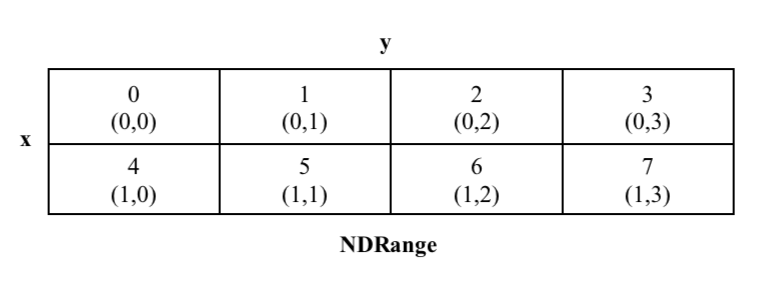
\includegraphics[width=8cm]{/home/ruoyong/paper1_2021_5/f1} }}%
    \qquad
    \subfloat[]{{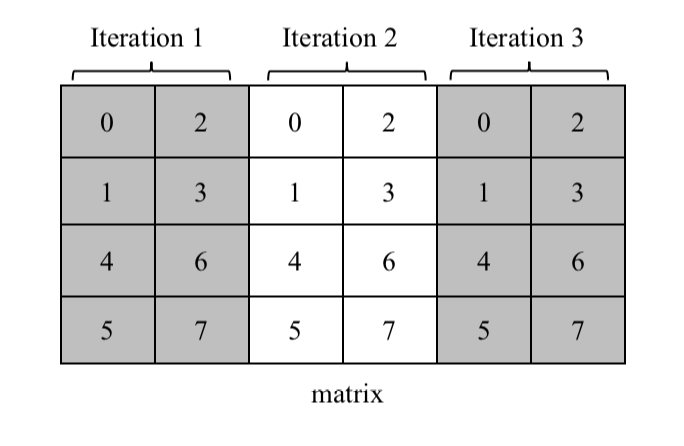
\includegraphics[width=8cm]{/home/ruoyong/paper1_2021_5/f2} }}%
    \caption{name?\label{fig:1}}%
\end{figure}

Now we use the 4 streams created in Section 2.1 and an NDRange of 1 by 4 work items to generate a vector \code{sim_1} of 6 i.i.d. $U (0,1)$ random numbers using the function \fct{gpuRandom::runif}. If \code{streams} and \code{Nglobal} are both missing, then by default \code{Nglobal} is set as (64,8), and a `vclMatrix' of \code{prod(Nglobal)} streams is supplied. The output is an S4 object (a `\code{vclVector}' or a `\code{vclMatrix}'), to view the generated random numbers, we need to convert it to an R vector or matrix, in this way, the random numbers are moved from the global memory of device to the host.
\begin{knitrout}
\definecolor{shadecolor}{rgb}{1, 1, 1}\color{fgcolor}\begin{kframe}
\begin{verbatim}
sim_1 = gpuRandom::runif(n = 6, streams = streams1, Nglobal = c(1, 4),
    type = "double")
as.vector(sim_1)
## [1] 0.7353245 0.5180770 0.6142074 0.2319392 0.1100781 0.3619766
\end{verbatim}
\end{kframe}
\end{knitrout}
The arguments of the \fct{gpuRandom::runif} are described as follows:
\begin{itemize}
  \item \code{n}: a vector of length 2 specifying the row and column number if to create a matrix, or specifying the length if to create a vector.
  \item \code{streams}: streams used for random number generation.
  \item \code{Nglobal}: global index space that defines the total work-items that execute in parallel. Default is set as $(64,8)$.
  \item \code{type}: ``double'' or ``float'' format of generated random numbers.
\end{itemize}
Next we show that by using a same stream \code{streams2} as \code{streams1},  \fct{gpuRandom::runif} returns a vector \code{sim_2} of same random numbers as \code{sim_1}. 
\begin{knitrout}
\definecolor{shadecolor}{rgb}{1, 1, 1}\color{fgcolor}\begin{kframe}
\begin{verbatim}
sim_2 <- gpuRandom::runif(n = 6, streams = streams2, Nglobal = c(1, 4),
    type = "double")
as.vector(sim_2)
## [1] 0.7353245 0.5180770 0.6142074 0.2319392 0.1100781 0.3619766
\end{verbatim}
\end{kframe}
\end{knitrout}
Notice that \code{streams2} is a \code{deepcopy} of \code{streams1} before \code{streams1} is used. Reusing \code{streams1} will produce a vector different from \code{sim_1} (see \code{sim_3}). Because each time a random number is generated, the current state of the stream is changed (advances by one position), below shows the first six rows (current states) of \code{streams1} after it being used.
\begin{knitrout}
\definecolor{shadecolor}{rgb}{1, 1, 1}\color{fgcolor}\begin{kframe}
\begin{verbatim}
sim_3 = gpuRandom::runif(n = 6, streams = streams1, Nglobal = c(1, 4),
    type = "double")
as.vector(sim_3)
## [1] 0.6487742 0.1112075 0.3661944 0.5018562 0.1088229 0.3114331
t(as.matrix(streams1))[1:6, ]
##            [,1]       [,2]       [,3]       [,4]
## [1,] 1167281028  640923766  502033783  739421137
## [2,] 1918428443 1912157188 1322587635 1475938232
## [3,] 1858462085  286315187 1964121530  730262207
## [4,]  933585541 2119609883 1949818481 1630192198
## [5,] 1132031887  834429287 1607232546  324551134
## [6,]  465230163   47498872 1462898381  795289868
\end{verbatim}
\end{kframe}
\end{knitrout}
Unlike the objects created by \proglang{R}, by default they remain in the memory after a restart. Streams created on GPU does not remain in the memory when a new \proglang{R} session begins. However, we can save the streams on the CPU in a file using the \fct{save} function, and later recall the streams with the \fct{load} function, in this way we can reproduce the same sequence of random numbers in simulations. Below is a trivial example, in which we demonstrate saving \code{streams1} to a data file called \code{streams_from_GPU.rds} on CPU and then load it back and transfer it to GPU to produce the vector called \code{sim_saved}, which is also the same as \code{sim_1}.
\begin{knitrout}
\definecolor{shadecolor}{rgb}{1, 1, 1}\color{fgcolor}\begin{kframe}
\begin{verbatim}
saveRDS(streams_from_GPU, "streams_from_GPU.rds")
\end{verbatim}
\end{kframe}
\end{knitrout}
\begin{knitrout}
\definecolor{shadecolor}{rgb}{1, 1, 1}\color{fgcolor}\begin{kframe}
\begin{verbatim}
# Load the streams object as streams_saved
streams_saved <- gpuR::vclMatrix(readRDS("streams_from_GPU.rds"))
sim_saved = gpuRandom::runif(n=6,streams=streams_saved, 
                             Nglobal=c(1,4), type="double")
as.vector(sim_saved)
## [1] 0.7353245 0.5180770 0.6142074 0.2319392 0.1100781 0.3619766
\end{verbatim}
\end{kframe}
\end{knitrout}

We evaluate the distribution of 50000 GPU-generated double-precision uniform random numbers by making a density histogram  (the left panel in Figure \ref{fig0}), and plotting its empirical cumulative distribution and overlaying the theoretical cumulative distribution (the right panel in Figure \ref{fig0}). The two cumulative distribution lines seem to overlap completely, suggesting the data generated by \fct{gpuRandom::runif} does come from a standard uniform distribution.
\begin{knitrout}
\definecolor{shadecolor}{rgb}{1, 1, 1}\color{fgcolor}\begin{kframe}
\begin{verbatim}
streams <- CreateStreamsGpu(Nstreams =512, keepInitial=1)
random_vector<-gpuRandom::runif(n=50000, streams=streams, 
                                Nglobal=c(64,8), type="double")
random_vector<-as.vector(random_vector)
\end{verbatim}
\end{kframe}
\end{knitrout}
\begin{figure}[H]
\centering
\begin{knitrout}
\definecolor{shadecolor}{rgb}{1, 1, 1}\color{fgcolor}
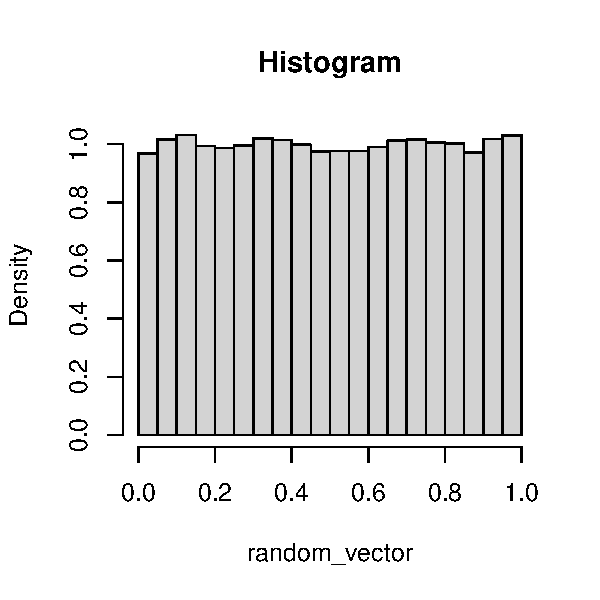
\includegraphics[width=0.45\textwidth]{figure/largenumberuniforms-1} 
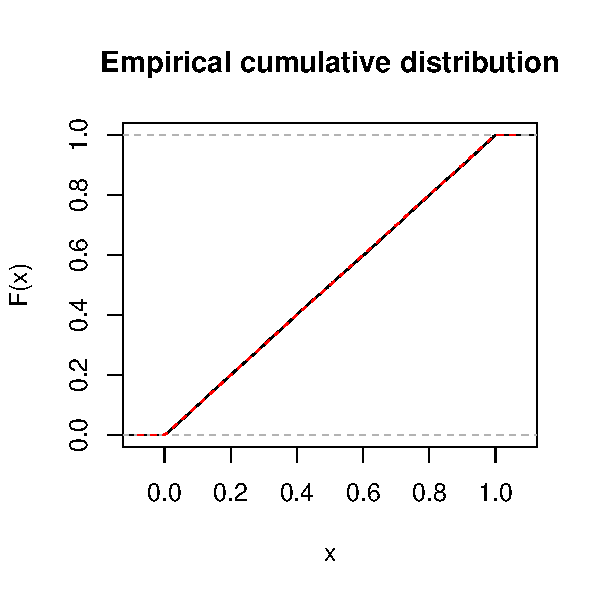
\includegraphics[width=0.45\textwidth]{figure/largenumberuniforms-2} 
\end{knitrout}
\caption{histogram and empirical cumulative distribution of the GPU-generated random numbers.\label{fig0}}
\end{figure}











\subsection{Using streams to generate i.i.d. N (0, 1) random numbers on GPU}
We apply the Box-Muller transformation to $U (0,1)$ random numbers to generate Gaussian random numbers. As shown in Algorithm \ref{algorithm1}, Box-Muller algorithm takes two independent, standard uniform random variables $U_1$ and $U_2$ and produces two independent, standard Gaussian random variables $X$ and $Y$, where $R$ and $\Theta$ are polar coordinate random variables. The derivation basically uses transformation from Cartesian coordinates to polar coordinates to represent two independent, Normally distributed random variables. The Box-Muller algorithm turns out to be the best choice for Gaussian transform on GPU compared to other transform methods \citep{howes2007efficient}, because this algorithm has no branching or looping, which are the things GPU is not good at, but GPU is good at the high computational load of sine and cosine functions in the algorithm. 

\begin{algorithm*}[H] \label{algorithm1}
\SetAlgoLined
 1, Generate $U_1$, $U_2$ i.i.d. from $U (0,1)$ \;
 2, Define \begin{align*} 
& R = \sqrt{-2*\log U_1},\\
&  \Theta = 2\pi*U_2,\\
&  X=R*\cos(\Theta),\\
& Y=R*\sin(\Theta);\;\end{align*}
 3, Take $X$ and $Y$ as two independent draws from $N(0,1)$\;
 \caption{Box-Muller algorithm.}
\end{algorithm*}


Listing \ref{lst:normal} shows a fragment of the kernel that generates standard Gaussian random numbers. Aside from using local memory and the part that does the Box-Muller transformation, this kernel is the same with the kernel for generating uniform random numbers shown in Listing \ref{lst:uniformkernel}. If developers want to use other Gaussian transform methods, this kernel is easy to be modified and incorporated in other \proglang{R} packages. The kernel executes over a 2-dimensional index space of $1 \times 2$ work-groups. \code{part[0]} and \code{part[1]} correspond to $R$ and $\Theta$ in the formulas respectively. As the work-items in each work-group proceed at differing rates, \code{barrier(CLK_LOCAL_MEM_FENCE)} ensures correct ordering of memory operations to local memory, so that Gaussian random numbers $(X_1,Y_1), (X_2,Y_2), \dots, (X_n,Y_n)$ are generated in pairs correctly, errors such as $(X_n, Y_{(n-1)})$ or $(X_{(n-1)}, Y_{(n)})$ are avoided.
%
\begin{framed}
\begin{lstlisting}[language=C,basicstyle=\small,caption={name},label={lst:normal}]
const int 
index = get_global_id(0)*get_global_size(1) + get_global_id(1);
const int 
DrowInc = 2*get_global_size(0), DrowStartInc = DrowInc * NpadCol;
int Drow, Dcol, DrowStart, Dentry;
uint temp;
uint g1[3], g2[3];
const int startvalue=index * NpadStreams;

local double part[2], cosPart1, sinPart1;

streamsToPrivate(streams,g1,g2,startvalue);

// Iterate for the rows
for(Drow=2*get_global_id(0), 
    DrowStart = (Drow + get_local_id(1))* NpadCol;
    Drow < Nrow; 
    Drow += DrowInc, DrowStart += DrowStartInc) {
  // Iterate for the columns
  for(Dcol=get_group_id(1), Dentry = DrowStart + Dcol;
      Dcol < Ncol;
      Dcol += get_num_groups(1), Dentry += get_num_groups(1)) {
    
    // Generates an uniform random integer
    temp = clrngMrg31k3pNextState(g1, g2);
    
    if(get_local_id(1)) {
      // Cache data to local memory
      part[1] = TWOPI_mrg31k3p_NORM_cl * temp;
      cosPart1 = cos(part[1]);
      sinPart1 = sin(part[1]);
    } else {
      part[0] = sqrt(-2.0*log(temp * mrg31k3p_NORM_cl));
    }
    
    // Wait until all work items have read the data and 
    // it becomes visible
    barrier(CLK_LOCAL_MEM_FENCE);
    
    // Perform the operation and output the data
    if(get_local_id(1)) {
      out[Dentry] = part[0]*sinPart1;
    } else {
      out[Dentry] = part[0]*cosPart1;
    }
    
    barrier(CLK_LOCAL_MEM_FENCE);
    
  }//Dcol
}//Drow

streamsFromPrivate(streams,g1,g2,startvalue);
\end{lstlisting}
\end{framed}
We illustrate in Figure \ref{fig3} how this kernel executes in practice with the previous toy example: to create a $4 \times 6$ matrix of Gaussian random numbers using a $2 \times 4$ NDRange and 8 streams. Work items are organized to be 1 by 2 work groups as Gaussian numbers are generated in pairs using the Box-Muller method. The shading on the grids in the NDRange distinguishes work groups. Each work group generates a pair of Gaussian random numbers \code{(X,Y)} in each iteration, where work item of `\code{get_local_id(1)}$=0$' generates the \code{X} of a pair, and work item of `\code{get_local_id(1)}$=1$' generates the \code{Y} of a pair. The numbers in the third row in each gird of NDRange represents the local index of each work item. Here with the loop iterating over columns, the cells of matrix are filled from left to right, that is, in the first iteration, the 8 work items generate random numbers in the leftmost two columns (8 cells) of matrix simultaneously, the second iteration fills random numbers in the middle two columns of the matrix, and the third iteration fills the rest two columns of the matrix simultaneously. Therefore, each work item generates one Gaussian random number in each iteration, the matrix filling process is the same as that shown in Figure \ref{fig:1}. 

\begin{figure}[H]%
    \centering
    \subfloat[]{{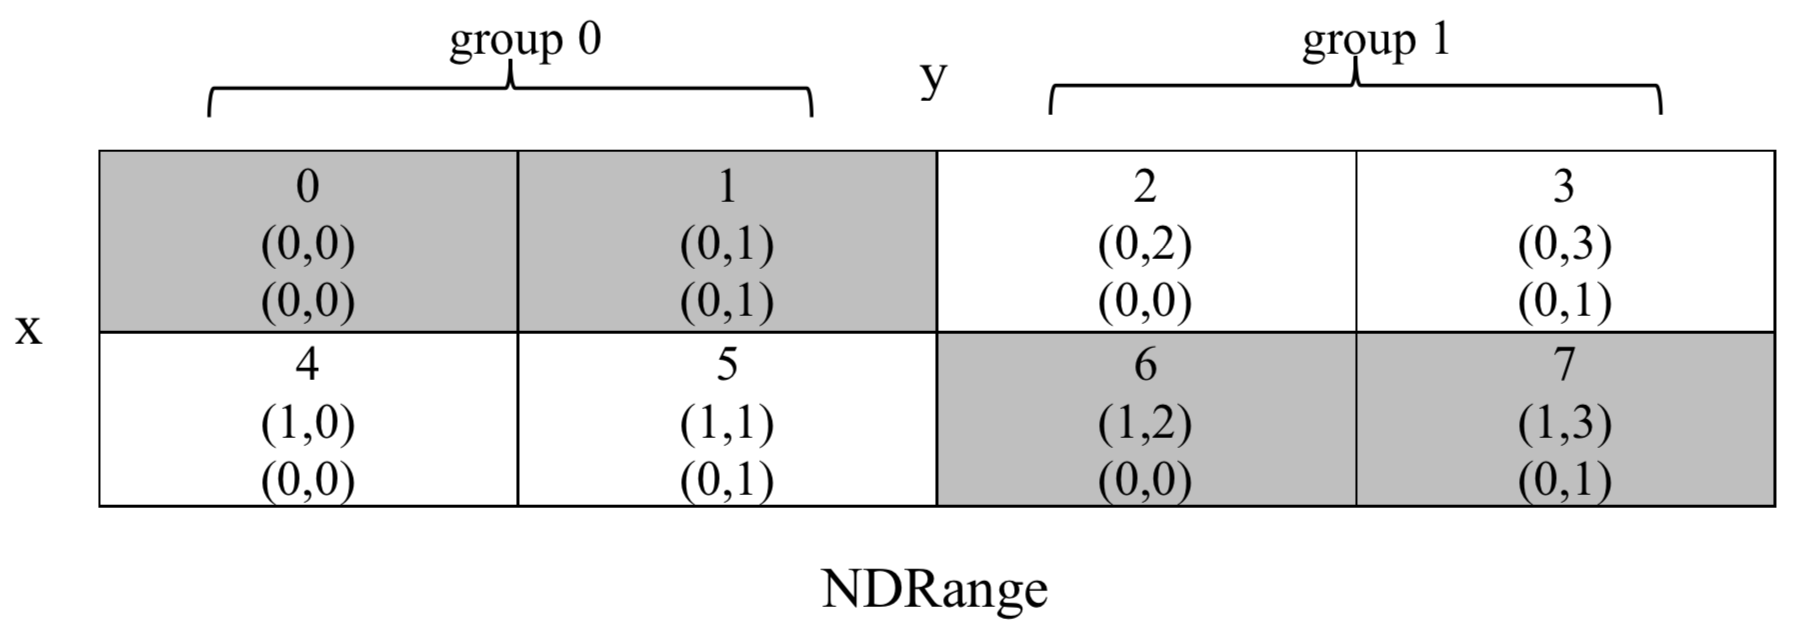
\includegraphics[width=8cm]{/home/ruoyong/paper1_2021_5/f3} }}%
    \qquad
    \subfloat[]{{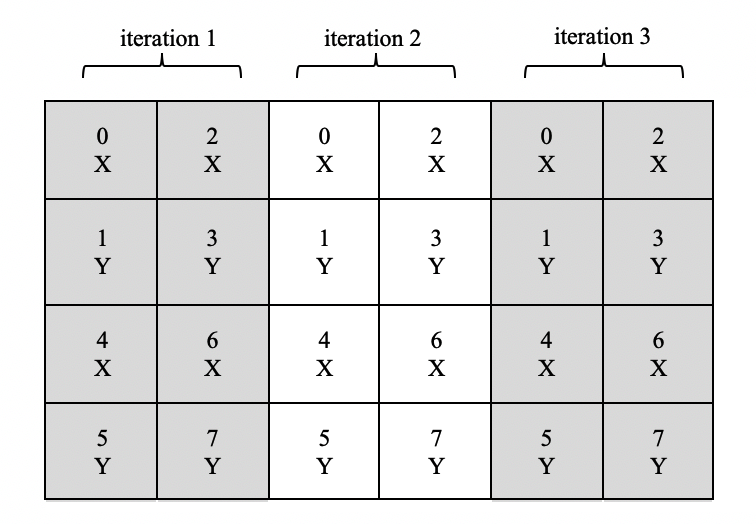
\includegraphics[width=8cm]{/home/ruoyong/paper1_2021_5/f4} }}%
    \caption{name???}%
    \label{fig3}
\end{figure}
 

In the following code, We create a $1024 \times 512$ matrix named \code{normal_matrix} of single-precision floating-point Gaussian random numbers, and assess Normality by making a histogram and a Q-Q plot of the generated random numbers in Figure \ref{fig2}. The points in the Q-Q plot shown in the right panel of Figure \ref{fig2} fall along the diagonal line, we have good evidence the generated data are from Gaussian distribution. We find doing a Q-Q plot can occupy a large amount of time in the process of producing an R markdown file, so as an incidental work, we adapted the \proglang{R} function \fct{stat::qnorm} to make the function \fct{gpuRandom::qqnorm} that does the quantile computation for the normal distribution part on GPU, which can speed up the Q-Q plot greatly.
\begin{knitrout}
\definecolor{shadecolor}{rgb}{1, 1, 1}\color{fgcolor}\begin{kframe}
\begin{verbatim}
streams <- CreateStreamsGpu(Nstreams =512*128, keepInitial=1)
normal_matrix<-gpuRandom::rnorm(c(1024,512), streams=streams, 
                                Nglobal=c(512,128), type="float")
\end{verbatim}
\end{kframe}
\end{knitrout}
\begin{knitrout}
\definecolor{shadecolor}{rgb}{1, 1, 1}\color{fgcolor}\begin{kframe}
\begin{verbatim}
avector<-as.vector(as.matrix(normal_matrix))
\end{verbatim}
\end{kframe}
\end{knitrout}
\begin{figure}[H]
\centering
\begin{knitrout}
\definecolor{shadecolor}{rgb}{1, 1, 1}\color{fgcolor}\begin{kframe}
\begin{verbatim}
hist(avector,breaks=40, main = "histogram")
gpuRandom::qqnorm(avector, Nglobal=c(128,64), main="Q-Q Plot")
\end{verbatim}
\end{kframe}
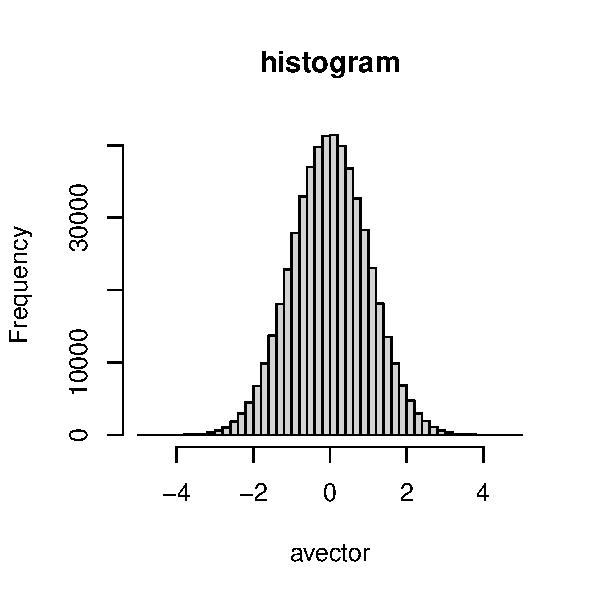
\includegraphics[width=0.45\textwidth]{figure/histAndQQ-1} 
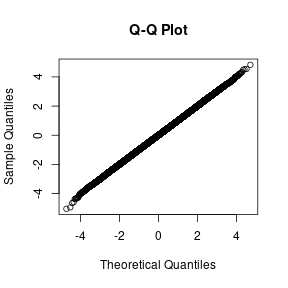
\includegraphics[width=0.45\textwidth]{figure/histAndQQ-2} 
\end{knitrout}
\caption{Histogram and Q-Q plot of the GPU-generated random numbers.\label{fig2}}
\end{figure}

We generate a large-size matrix of 100 million double-precision Gaussian random numbers, and compare the runtime between using \fct{stats::rnorm} and \fct{gpuRandom::rnorm}. Both process are not time-consuming, however, using \fct{gpuRandom::rnorm} with $512 \times 128$ work-items is around 120 times (the number may fluctuate a bit from executions) faster than using the \fct{stats::rnorm}. The difference in elapsed time becomes larger when matrix size goes larger.
\begin{knitrout}
\definecolor{shadecolor}{rgb}{1, 1, 1}\color{fgcolor}\begin{kframe}
\begin{verbatim}
system.time(gpuRandom::rnorm(c(10000,10000), streams=streams, 
                             Nglobal=c(512,128), type="double"))
##    user  system elapsed 
##   0.140   0.004   0.143
system.time(matrix(stats::rnorm(10000^2),10000,10000))
##    user  system elapsed 
##   6.610   0.862   7.466
\end{verbatim}
\end{kframe}
\end{knitrout}










\section{Monte Carlo simulation for Fisher's exact test}
One application of GPU-generated random numbers in \pkg{gpuRandom} is Monte Carlo simulation for Fisher's exact test. Fisher’s exact test is usually applied for analyzing $2 \times 2$ contingency tables when one of the expected values in table is less than 5. Different from methods which rely on approximation, Fisher's exact test computes directly the probability of obtaining each possible combination of the data for the same row and column totals (marginal totals) as the observed table, and get the exact p-value by adding together all the probabilities of tables as extreme or more extreme than the one observed. However, when the observed table gets large in terms of sample size and table dimensions, the number of combinations of cell frequencies with the same marginal totals gets very large, \cite[][p. 23]{mehta2011ibm} shows a $5 \times 6$ observed table that has 1.6 billion possible tables. Calculating the exact P-values may lead to very long running time and can sometimes exceed the memory limits of your computer. Hence, the option \code{simulate.p.value = TRUE} in \fct{stats::fisher.test} is provided, which enables computing p-values by Monte Carlo simulation for tables larger than 2 $\times$ 2. Given an observed table and a number of replicates $B$, the Monte Carlo simulation does the following steps: 
\begin{enumerate}
  \item Calculate the test statistic for the observed table.
	\item In each iteration, simulate a random table with the same dimensions and marginal totals as the observed table, compute and sometimes save the test statistic (minus log-factorial of table) from the random table.
	\item Count the number of iterations (\emph{Counts}) that have test statistics less or equal to the one from the observed table.
	\item Estimate p-value using $\frac{1 + \emph{Counts}}{B + 1}$.
\end{enumerate}
The Monte Carlo simulation solves the computational problem of Fisher's exact test but can still take long running time when $B$ reaches millions in scale, thus we make the function \fct{gpuRandom::fisher.sim} that does the steps 1, 2 and 3 parallelly on GPU, and step 2 of saving the test statistics from the random tables as an option in \fct{gpuRandom::fisher.sim}, which largely saves processing time. 

We show the usage and advantage of \fct{gpuRandom::fisher.sim} by computing the p-values for two real data examples: one with a relatively big p-value and another with a very small p-value, and compare the runtime with using \fct{stats::fisher.test} for each of the data sets on two computers: one with a very good CPU and an ordinary GPU, the other is equipped with an excellent GPU and an ordinary CPU. The \proglang{R} outputs for testing on computer 2 is shown in the following. 

% \begin{table}[H]
% \begin{tabular}{ |c|c|c|c|c|c| } 
% \hline
%            & host   &                     device \\ \hline
%  Computer1 & INtel Xenon W-2145 3.7 Ghz & Amd Radeon VII  \\ \hline
%  Computer2 & VCPU Intel Xenon Skylake 2.5ghz & VGPU Nvidia Tesla V100 \\ \hline
% \end{tabular}
% \caption{ Device information for run-time compare.\label{tab:device}}
% \end{table}

The 2-way contingency table \ref{tab:month} and table \ref{tab:week} consist of selected data from the 2018 Natality public use file \citep{National2018} from the Centers for Disease Control and Prevention’s National Center for Health Statistics, the 2018 natality data file may be downloaded at \url{https://www.cdc.gov/nchs/data_access/VitalStatsOnline.htm}. The row variable of the first table represents the twelve months: from January to December, and for the second table it represents the seven weekdays: Monday to Sunday. The column variables of these two tables represent the twelve categories of congenital anomalies of the newborn: 1) Anencephaly; 2) Meningomyelocele/Spina bifida; 3) Cyanotic congenital heart disease; 4) Congenital diaphragmatic hernia; 5) Omphalocele; 6) Gastrochisis; 7) Limb reduction defect; 8) Cleft lip with or without cleft palate; 9) Cleft palate alone; 10) Down syndrome; 11) Suspected chromosomal disorder; and 12) Hypospadias.

\subsection{Comparing running time: Month data example}

\begin{knitrout}
\definecolor{shadecolor}{rgb}{1, 1, 1}\color{fgcolor}\begin{table}[H]

\caption{\label{tab:monthdata}Month\label{tab:month}}
\centering
\begin{tabular}[t]{l|r|r|r|r|r|r|r|r|r|r|r|r}
\hline
  & Ane & Men & Cya & Her & Omp & Gas & Lim & Cle & Pal & Down & Chro & Hypo\\
\hline
Jan & 29 & 55 & 172 & 46 & 39 & 73 & 48 & 183 & 77 & 103 & 102 & 174\\
\hline
Feb & 25 & 45 & 175 & 35 & 31 & 55 & 34 & 142 & 81 & 115 & 100 & 180\\
\hline
Mar & 31 & 48 & 182 & 41 & 47 & 72 & 40 & 200 & 86 & 90 & 96 & 180\\
\hline
Apr & 34 & 45 & 186 & 36 & 32 & 75 & 42 & 173 & 56 & 87 & 90 & 193\\
\hline
May & 33 & 40 & 187 & 46 & 24 & 80 & 35 & 180 & 75 & 91 & 100 & 197\\
\hline
Jun & 34 & 48 & 189 & 35 & 33 & 75 & 45 & 154 & 74 & 102 & 100 & 182\\
\hline
Jul & 26 & 43 & 198 & 34 & 21 & 74 & 36 & 179 & 79 & 86 & 92 & 193\\
\hline
Aug & 24 & 41 & 189 & 44 & 43 & 62 & 48 & 183 & 88 & 109 & 94 & 194\\
\hline
Sept & 34 & 44 & 147 & 40 & 37 & 66 & 36 & 158 & 73 & 112 & 103 & 196\\
\hline
Oct & 25 & 43 & 207 & 45 & 31 & 65 & 49 & 181 & 77 & 108 & 115 & 220\\
\hline
Nov & 36 & 55 & 188 & 39 & 39 & 62 & 43 & 144 & 68 & 98 & 79 & 173\\
\hline
Dec & 23 & 48 & 196 & 31 & 31 & 71 & 31 & 177 & 86 & 86 & 73 & 156\\
\hline
\end{tabular}
\end{table}

\end{knitrout}

\begin{knitrout}
\definecolor{shadecolor}{rgb}{1, 1, 1}\color{fgcolor}\begin{kframe}
\begin{verbatim}
#using CPU
stats::fisher.test(month,simulate.p.value = TRUE,B=1e6)$p.value
## [1] 0.4042196
system.time(stats::fisher.test(month,simulate.p.value = TRUE,B=1e6))
##    user  system elapsed 
##  14.578   0.002  14.569
\end{verbatim}
\end{kframe}
\end{knitrout}
\fct{stats::fisher.test} takes about 9.8 seconds (time varies a little bit from executions) for one million simulations, has a p-value of 0.4035.
\begin{knitrout}
\definecolor{shadecolor}{rgb}{1, 1, 1}\color{fgcolor}\begin{kframe}
\begin{verbatim}
almost.1 <- 1 + 64 * .Machine$double.eps
observed_m= -gpuRandom::logfactSum(month, c(16,16))/almost.1

month_GPU<-vclMatrix(month,type="integer")
result_monthgpu <- gpuRandom::fisher.sim(month_GPU, 1e6, streams=streams,
                   type="double", returnStatistics=TRUE,  Nglobal = c(128,128))
result_monthgpu$simNum
## [1] 1015808
result_monthgpu$counts
## [1] 410098
result_monthgpu$p.value
## [1] 0.4037166
\end{verbatim}
\end{kframe}
\end{knitrout}
We requested one million simulations on GPU while the actual number of simulation is 999424, and got 403274 cases whose test statitsic is below the observed threshold, so the p-value from \fct{gpuRandom::fisher.sim} for this table is about 0.40375, which is close enough to the p-value from \fct{stats::fisher.test}: 0.40380.  
\begin{knitrout}
\definecolor{shadecolor}{rgb}{1, 1, 1}\color{fgcolor}\begin{kframe}
\begin{verbatim}
#using GPU
system.time(gpuRandom::fisher.sim(month_GPU, 1e6, streams=streams, 
            type="double", returnStatistics=FALSE, Nglobal = c(128,128)))
##    user  system elapsed 
##   0.702   0.005   0.706
\end{verbatim}
\end{kframe}
\end{knitrout}
\fct{gpuRandom::fisher.sim} takes about 0.32 seconds, \pkg{gpuRandom} accounts for 2.2\% of the elapsed time on CPU. 



\subsection{Comparing running time: Week data example}


\begin{knitrout}
\definecolor{shadecolor}{rgb}{1, 1, 1}\color{fgcolor}\begin{table}[H]

\caption{\label{tab:weekdata}Week\label{tab:week}}
\centering
\begin{tabular}[t]{l|r|r|r|r|r|r|r|r|r|r|r|r}
\hline
  & Ane & Men & Cya & Her & Omp & Gas & Lim & Cle & Pal & Down & Chro & Hypo\\
\hline
Mon & 30 & 34 & 173 & 37 & 23 & 80 & 49 & 191 & 83 & 122 & 109 & 216\\
\hline
Tue & 60 & 121 & 383 & 80 & 83 & 131 & 71 & 349 & 146 & 164 & 168 & 352\\
\hline
Wed & 51 & 106 & 417 & 92 & 73 & 145 & 72 & 333 & 136 & 179 & 196 & 351\\
\hline
Thu & 60 & 86 & 362 & 69 & 74 & 120 & 85 & 326 & 132 & 220 & 187 & 359\\
\hline
Fri & 52 & 94 & 347 & 87 & 59 & 123 & 68 & 323 & 145 & 170 & 166 & 345\\
\hline
Sat & 52 & 63 & 323 & 67 & 64 & 135 & 73 & 316 & 170 & 189 & 188 & 357\\
\hline
Sun & 49 & 51 & 211 & 40 & 32 & 96 & 69 & 216 & 108 & 143 & 130 & 258\\
\hline
\end{tabular}
\end{table}

\end{knitrout}
We perform 10 million simulations for the ``week'' table.
\begin{knitrout}
\definecolor{shadecolor}{rgb}{1, 1, 1}\color{fgcolor}\begin{kframe}
\begin{verbatim}
#using CPU
fisher.test(week,simulate.p.value = TRUE,B=1e7)$p.value
## [1] 0.0001284
system.time(fisher.test(week,simulate.p.value = TRUE,B=1e7))
##    user  system elapsed 
##  90.259   0.150  90.439
\end{verbatim}
\end{kframe}
\end{knitrout}
The ``week'' table has a much smaller p-value: around 0.0001208, which should require a larger number of simulations to get a more accurate p-value.
\begin{knitrout}
\definecolor{shadecolor}{rgb}{1, 1, 1}\color{fgcolor}\begin{kframe}
\begin{verbatim}
observed_w= -gpuRandom::logfactSum(week, c(16,16))/almost.1

week_GPU<-gpuR::vclMatrix(week,type="integer")
result_weekgpu<-gpuRandom::fisher.sim(week_GPU, 1e7, streams=streams,
                type="double",returnStatistics=TRUE,Nglobal = Nglobal)
result_weekgpu$simNum
## [1] 10010624
result_weekgpu$counts
## [1] 1260
result_weekgpu$p.value
## [1] 0.0001259662
\end{verbatim}
\end{kframe}
\end{knitrout}
With about ten million simulations, we get 1223 cases and a p-value around 0.0001224705. We summarized the results in Table \ref{tab:summary}.
\begin{knitrout}
\definecolor{shadecolor}{rgb}{1, 1, 1}\color{fgcolor}\begin{kframe}
\begin{verbatim}
#using GPU
system.time(gpuRandom::fisher.sim(week_GPU, 1e7, streams=streams,
            type="double", returnStatistics=FALSE,Nglobal = Nglobal))
##    user  system elapsed 
##   4.477   0.009   4.483
\end{verbatim}
\end{kframe}
\end{knitrout}
\fct{stats::fisher.test} takes 90.1 seconds, while \fct{fisher.sim} takes about 1.90 seconds, the elapsed time is decreased to about 20\% of the time taken on CPU. 


\subsection{A summary of the results}
\begin{knitrout}
\definecolor{shadecolor}{rgb}{1, 1, 1}\color{fgcolor}\begin{table}[H]

\caption{\label{tab:summarycompare}Summary of comparions of Fisher's test simulation on different devices. Computer 1 is equipped with CPU Intel Xenon W-2145 3.7Ghz and AMD Radeon VII. Computer 2 is equipped with	VCPU Intel Xenon Skylake 2.5Ghz and VGPU Nvidia Tesla V100.\label{tab:summary}}
\centering
\begin{tabular}[t]{l|l|l|l|l|l}
\hline
\multicolumn{1}{c|}{ } & \multicolumn{2}{c|}{Computer 1} & \multicolumn{2}{c|}{Computer 2} & \multicolumn{1}{c}{ } \\
\cline{2-3} \cline{4-5}
B & Intel 2.5ghz & AMD Radeon & Intel 3.7ghz & NVIDIA V100 & Data\\
\hline
\multicolumn{6}{l}{\textbf{P-value}}\\
\hline
\hspace{1em}1m & 0.403804 & 0.403507 & 0.4035606 & 0.403507 & month\\
\hline
\hspace{1em}10m & 0.0001251 & 0.0001274 & 0.0001202 & 0.0001274 & week\\
\hline
\multicolumn{6}{l}{\textbf{Run-time}}\\
\hline
\hspace{1em}1m & 9.74 & 2.28 & 14.58 & 0.32 & month\\
\hline
\hspace{1em}10m & 60.19 & 10.82 & 90.38 & 1.89 & week\\
\hline
\end{tabular}
\end{table}

\end{knitrout}
% \begin{table}[H]
% \centering
% \begin{tabular}{ |c|c|c|c|c|c| } 
%  \hline
%  data &   B  & Intel CPU &  AMD GPU & NVIDIA GPU \\ \hline
%  Month & 1e6 & 0.403804 & 0.403507  & 0.403507     \\ \hline
%  Week &  1e7  & 0.0001251 & 0.0001274 & 0.0001274\\ \hline
% \end{tabular}
% \caption{ Summary of p-values obtained on different devices.\label{tab:summary}}
% \end{table}
% 
% 
% \begin{table}[H]
% \centering
% \begin{tabular}{ |c|c|c|c|c|c| } 
%  \hline
%  data &   B  & Intel CPU & sencha CPU & AMD GPU & NVIDIA GPU \\ \hline
%  Month & 1e6 & 9.74 & 14.58 & 2.28 & 0.31\\ \hline
%  Week &  1e7  & 60.19 & 90.38 & 10.82 & 1.90\\ \hline
% \end{tabular}
% \caption{ Run-time compare of Fisher's test simulation on different devices, all numbers are in seconds.\label{tab:compare time}}
% \end{table}

Figure \ref{fig4} visualizes the approximate sampling distributions of the test statistics from the two examples "Month" and "Week", by plotting a histogram for each of the example. The values of observed statistics are calculated by \fct{gpuRandom::logfactSum} and are marked with a blue line on each plot. 
\begin{figure}[H]
\centering
\begin{knitrout}
\definecolor{shadecolor}{rgb}{1, 1, 1}\color{fgcolor}
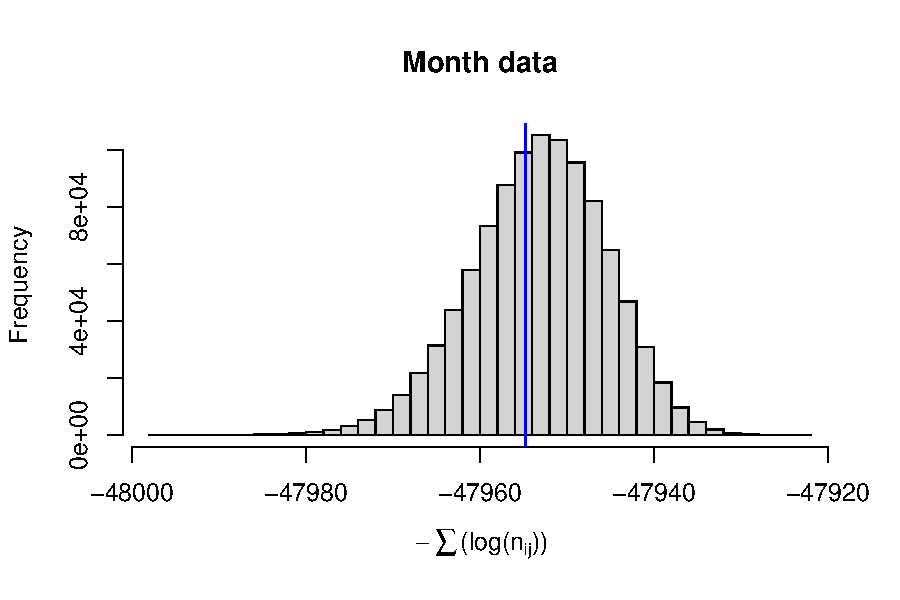
\includegraphics[width=0.45\textwidth]{figure/fighistMonth-1} 
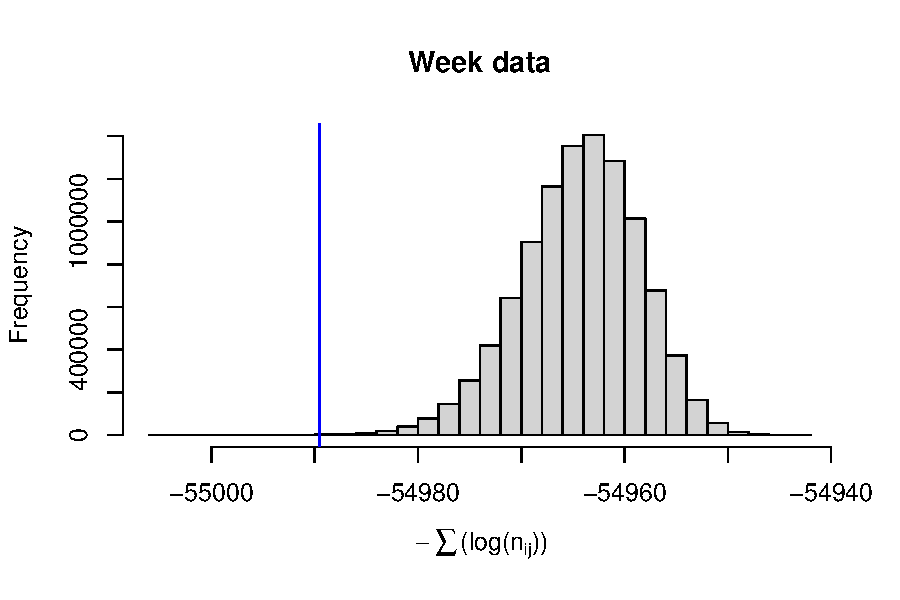
\includegraphics[width=0.45\textwidth]{figure/fighistMonth-2} 
\end{knitrout}
\caption{ Frequency distribution for test statistics from month and week data tables.\label{fig4}}
\end{figure}







\section{Generating Gaussian random fields} 
Given a parameter space $X$, a random field $U$ on $X$ is a collection of random variables $\{U_x :x\in X\}$. A Gaussian random field is a random field with the property that for any positive integer $n$ and any set of locations $x_1,\dots,x_n \in X$, the joint distribution of $U=(U_{x_1},\dots,U_{x_n})$ is multivariate Gaussian. One reason that Gaussian random fields play an important role is that the specification of their finite-dimensional distributions is simple \citep{abrahamsen1997review}, the expectation $\mu(x)$ and covariance function $\Sigma$ completely determine the distribution of $U$, where 
\begin{gather*} 
\mu(x) = \E (U(x)),\\
\Sigma_{ij} = \cov (U(x_i),U(x_j)).
\end{gather*}
There exist many choices for the covariance function $\Sigma$, one common choice is the Mat\'ern covariance function \citep{matern1960spatial}. The Mat\'ern covariance between $U(x)$ and $U(x')$ takes the form 
\begin{equation*}
\Sigma(d;\sigma^2,\phi,\kappa)=\sigma^2*\frac{2^{\kappa-1}}{\Gamma(\kappa)} (\sqrt{8\kappa} \frac{d}{\phi})^\kappa  K_\kappa(\sqrt{8\kappa}  \frac{d}{\phi}),  \quad \text{where} \quad \phi 	\geq 0,  \kappa 	\geq 0,
\end{equation*} 
$d =\|x-x'\|$ is the Euclidean distance between two spatial points, 
$\sigma^2$ the variance of the random field $U$.
$\Gamma(\cdot)$ is the standard gamma function,  $\phi$ is the range parameter or scale parameter with the dimension of distance, it controls the rate of decay of the correlation as $d$ increases. $K_\kappa(\cdot)$ is the modified Bessel function of the second kind with order $\kappa$, $\kappa$ is the shape parameter which determines the smoothness of $U(x)$, specifically, $U(x)$ is $m$ times mean-square differentiable if and only if $\kappa > m$. (For $\kappa=0.5$, the Mat\'ern covariance function reduces to the exponential covariance function $\sigma^2*\exp(-d/\phi)$, when $\kappa \rightarrow \infty$, $\Sigma(d) \rightarrow \sigma^2*\exp{-(\|d\|/\phi)^2}$, which is called the Gaussian covariance.)  There are several alternative parameterisations of Mat\'ern covariance functions appeared in literatures  \citep[see][]{haskard2007anisotropic}. In \pkg{gpuRandom}, we use the above form for computing Mat\'ern covariance.


Due to the importance of Gaussian random field, there are a large amount of studies devoted to Gaussian random field generation techniques. \cite{LiuandLi2019} gives a comprehensive review on 7 popular methods for Gaussian random field generation, which are the turning bands method \citep{matheron_1973}, spectral method \citep{Meja1974OnTS,1972JSV}, matrix decomposition method \citep{davis1987}, Karhunen-Lo\'eve expansion \citep{LoeveM:1978}, moving average method \citep{journel1974, oliver1995moving}, sequential simulation \citep{johnson1987multivariate, gomez1993joint, pebesma2004multivariable}, and local average subdivision \citep{fenton1990simulation}. All of these methods except matrix decomposition method, are approximations and has specific requirements on the type of grid or covariance functions. The matrix decomposition method is exact, it works for all covariance functions and can generate random field on all types of grids. Other \proglang{R} packages that offer simulation of Gaussian random fields like \pkg{geoR} \citep{geoR2001}, does not work for large number of locations; the \pkg{RandomFields} \citep{RandomFields2015,RandomFields2020} package can use different methods for simulation of Gaussian fields, among which the (modified) circulant embedding method \citep{Dietrich1997FastAE} for covariance matrix decomposition is also an exact method (need to confirm???), however, it works only for isotropic Gaussian fields and on rectangular grids. \pkg{gpuRandom} does exact simulation of exact Gaussian fields on the GPU as it relies on the matrix decomposition method. The implementation of this method is as follows.


Suppose $U=(U_1, U_2, \dots, U_n)$ is a Gaussian random field with mean $\mu$ and covariance matrix $\Sigma$, without loss of generality, we assume mean value zero $(\mu = 0)$. Since covariance matrix $\Sigma$ is symmetric and positive-definite, we can take Cholesky decomposition of $\Sigma$, then we can simulate random samples from $U$ using $U=L*D^{1/2}*Z$, where 
\begin{itemize}
\item $L$ is the lower unit triangular matrix in Cholesky decomposition of $\Sigma = L*D*L^\top$,
\item $D$ is a diagonal matrix.
\item $Z=(Z_1, Z_2, \dots, Z_n) \sim \text{MVN}(0,I_n)$, where $I_n$ is a $n \times n$ identity matrix.
\end{itemize}
The matrix decomposition method is straightforward to implement, however, when a large number ($n$) of locations is involved, the cost of Cholesky decomposition of the covariance matrix is $\mathcal{O}(n^3)$,  and the cost of matrix-vector multiplication $L*Z$ to generate the random field $U$ is $\mathcal{O}(n^2)$ \citep{LiuandLi2019}.  \pkg{gpuRandom} package takes advantage of GPU's parallel computing power to not only do the matrices decomposition (Cholesky decomposition and matrix-vector multiplication) in parallel, but also computes the covariance matrices in parallel on GPU. The following shows an example, in which we simulate 10 Gaussian random fields of mat\'ern covariance with 5 sets of parameters at one time, and introduces several GPU functions used in the simulation process.

\subsection{Simulating Gaussian random fields with Mat\'ern covariances}

Step 1, set up a $60 \times 80$ raster and coordinates on the raster, convert the matrix of coordinates \code{coordsSp@coords} to a ``vclMatrix'' object for later use.
\begin{knitrout}
\definecolor{shadecolor}{rgb}{1, 1, 1}\color{fgcolor}\begin{kframe}
\begin{verbatim}
Ngrid = c(60, 80)
NlocalCache = 1000
Nglobal = c(128, 64, 2)
Nlocal = c(4, 2, 2)
theType = "double"

myRaster = raster::raster( raster::extent(0,Ngrid[1]/Ngrid[2],5,6),Ngrid[1], Ngrid[2])
coordsSp = sp::SpatialPoints(raster::xyFromCell(myRaster, 1:raster::ncell(myRaster)))
coordsGpu = vclMatrix(coordsSp@coords, 
                      nrow(coordsSp@coords), 
                      ncol(coordsSp@coords), type=theType)
\end{verbatim}
\end{kframe}
\end{knitrout}
Step 2, create 5 parameter sets as a small example, in practical studies, there can be hundreds or thousands of parameter sets. Then, convert the matrix of parameters to a ``vclMatrix'' for later use by \fct{gpuRandom::maternGpuParam}.

\begin{knitrout}
\definecolor{shadecolor}{rgb}{1, 1, 1}\color{fgcolor}\begin{kframe}
\begin{verbatim}
myParamsBatch
##      shape range variance nugget anisoRatio anisoAngleRadians
## [1,]  1.25  0.50      1.5      0          1         0.0000000
## [2,]  2.15  0.25      2.0      0          4         0.4487990
## [3,]  0.55  1.50      2.0      0          4         0.4487990
## [4,]  2.15  0.50      2.0      0          4        -0.4487990
## [5,]  2.15  0.50      2.0      0          2         0.7853982
paramsGpu = gpuRandom::maternGpuParam(myParamsBatch, type=theType)
\end{verbatim}
\end{kframe}
\end{knitrout}
Step 3, compute Mat\'ern covariance matrices using \fct{gpuRandom::maternBatch}, the returned Mat\'ern covariance matrices %$\Sigma_1, \Sigma_2, \dots, \Sigma_5$ correspond to the 5 parameter sets respectively, the matrices 
are each of size $4800 \times 4800$ and are stacked by row in the output \code{maternCov}. 
\begin{knitrout}
\definecolor{shadecolor}{rgb}{1, 1, 1}\color{fgcolor}\begin{kframe}
\begin{verbatim}
maternCov = vclMatrix(0, nrow(paramsGpu)*nrow(coordsGpu), 
                         nrow(coordsGpu),type=theType)
dim(maternCov)
## [1] 24000  4800
gpuRandom::maternBatch(maternCov, coordsGpu, paramsGpu,
                       Nglobal=c(128,64), Nlocal=c(16,4))
\end{verbatim}
\end{kframe}
\end{knitrout}
Step 4, the first argument \code{maternCov} in \fct{gpuRandom::cholBatch} specifies the matrix object to take Cholesky decomposition. Unit lower triangular matrices $L_i$'s are returned and stacked by row in \code{maternCov}, \code{diagMat} stores the diagonal values of each $D_i$ in a row, for example, if each batch $\Sigma_i$ is of size $n \times n$, then each batch $L_i$ is $n \times n$, and each batch $D_i$ is $1 \times n$.
\begin{knitrout}
\definecolor{shadecolor}{rgb}{1, 1, 1}\color{fgcolor}\begin{kframe}
\begin{verbatim}
diagMat = vclMatrix(0, nrow(paramsGpu), ncol(maternCov), type = theType)
gpuRandom::cholBatch(maternCov, diagMat, numbatchD=nrow(myParamsBatch),
                     Nglobal= c(512, 8),
                     Nlocal= c(128, 8),
                     NlocalCache=2000)
\end{verbatim}
\end{kframe}
\end{knitrout}
% \begin{gather}
% \begin{bmatrix} \Sigma_{1} \\ \Sigma_2 \\ \Sigma_3 \\ \vdots
% \end{bmatrix}
%  \rightarrow
%  \begin{bmatrix}
%   L_{1} \\ L_{2} \\L_{3} \\ \vdots
%   \end{bmatrix} \text{and}
%   \begin{bmatrix}
%   D_{1} \\ D_{2} \\D_{3} \\ \vdots
%   \end{bmatrix}
% \end{gather}
Step 5, generate 2 standard Gaussian random vectors \code{zmatGpu}$=(Z_1, Z_2)$ using \fct{gpuRandom::rnorm}, in which \code{c(nrow(materCov),2)} specifies the number of rows and columns of \code{zmatGpu}.
\begin{knitrout}
\definecolor{shadecolor}{rgb}{1, 1, 1}\color{fgcolor}\begin{kframe}
\begin{verbatim}
streamsGpu <- gpuRandom::CreateStreamsGpu(Nstreams=128*64, keepInitial=TRUE)
\end{verbatim}
\end{kframe}
\end{knitrout}
\begin{knitrout}
\definecolor{shadecolor}{rgb}{1, 1, 1}\color{fgcolor}\begin{kframe}
\begin{verbatim}
zmatGpu = gpuRandom::rnorm(c(nrow(maternCov),2), 
                           streams=streamsGpu, Nglobal=c(128,64),
                           type = theType)
\end{verbatim}
\end{kframe}
\end{knitrout}
Step 6, use \fct{gpuRandom::multiplyLowerDiagonalBatch} to compute $U = L * D^{(1/2)}* Z$ in batches, see the following illustration. \code{simMat} is the output matrix for $U$, \code{maternCov}, \code{diagMat}, and \code{zmatGpu} correspond to the matrices of $L$, $D$ and $Z=(Z_1, Z_2)$ respectively.
\begin{knitrout}
\definecolor{shadecolor}{rgb}{1, 1, 1}\color{fgcolor}\begin{kframe}
\begin{verbatim}
simMat = vclMatrix(0, nrow(zmatGpu), ncol(zmatGpu), 
                   type = theType)

gpuRandom::multiplyLowerDiagonalBatch(
  simMat, maternCov, diagMat, zmatGpu,
  diagIsOne = 1L, # diagonal of L is one
  transformD = "sqrt", # take the square root of each element of D
  Nglobal,
  Nlocal,
  NlocalCache)
\end{verbatim}
\end{kframe}
\end{knitrout}
\begin{gather}
 \begin{bmatrix}  L_{1} \\ L_{2} \\L_{3} \\ \vdots
 \end{bmatrix} 
 *
  \begin{bmatrix}
   D_{1} \\ D_{2} \\D_{3} \\ \vdots
   \end{bmatrix} 
   *
   \begin{bmatrix}
   Z_{11} & Z_{12}
   \end{bmatrix}
  =
 \begin{bmatrix}
   L_1D_1Z_{11} & L_1D_1Z_{12} \\
   L_2D_2Z_{11} & L_2D_2Z_{12} \\
   L_3D_3Z_{11} & L_3D_3Z_{12} 
  \end{bmatrix}
\end{gather}
Step 7, Finally, plot the 10 simulated Gaussian random surfaces.
\begin{knitrout}
\definecolor{shadecolor}{rgb}{1, 1, 1}\color{fgcolor}\begin{kframe}
\begin{verbatim}
library(raster)
simRaster = brick(myRaster, nl = ncol(simMat)*nrow(paramsGpu))
values(simRaster) = as.vector(as.matrix(simMat))
names(simRaster) = apply(expand.grid('par',1:nrow(paramsGpu), 
                                     'sim', 1:ncol(simMat)), 1, paste, collapse='')
\end{verbatim}
\end{kframe}
\end{knitrout}
\begin{figure}[H]
\centering
\begin{knitrout}
\definecolor{shadecolor}{rgb}{1, 1, 1}\color{fgcolor}\begin{kframe}
\begin{verbatim}
par(mar=rep(0.1, 4))
for(D in names(simRaster)) {
  plot(extent(simRaster))
  plot(simRaster[[D]], legend=FALSE, add=TRUE)
}
\end{verbatim}
\end{kframe}
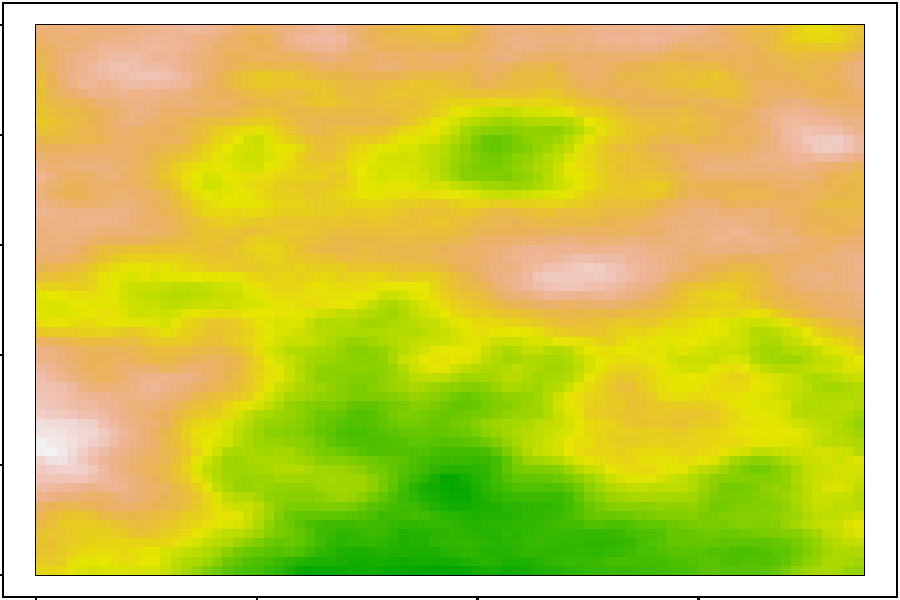
\includegraphics[width=0.45\textwidth]{figure/maternplot-1} 
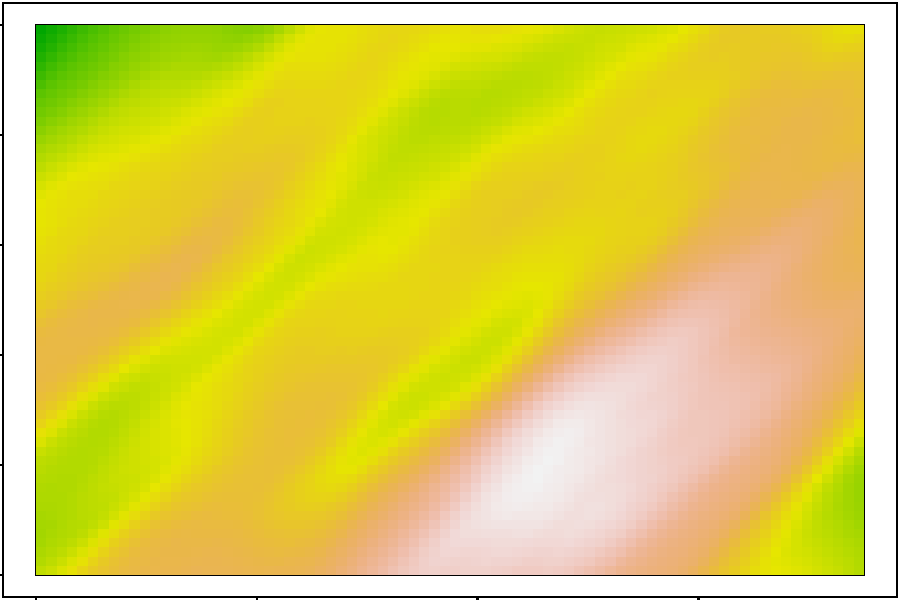
\includegraphics[width=0.45\textwidth]{figure/maternplot-2} 
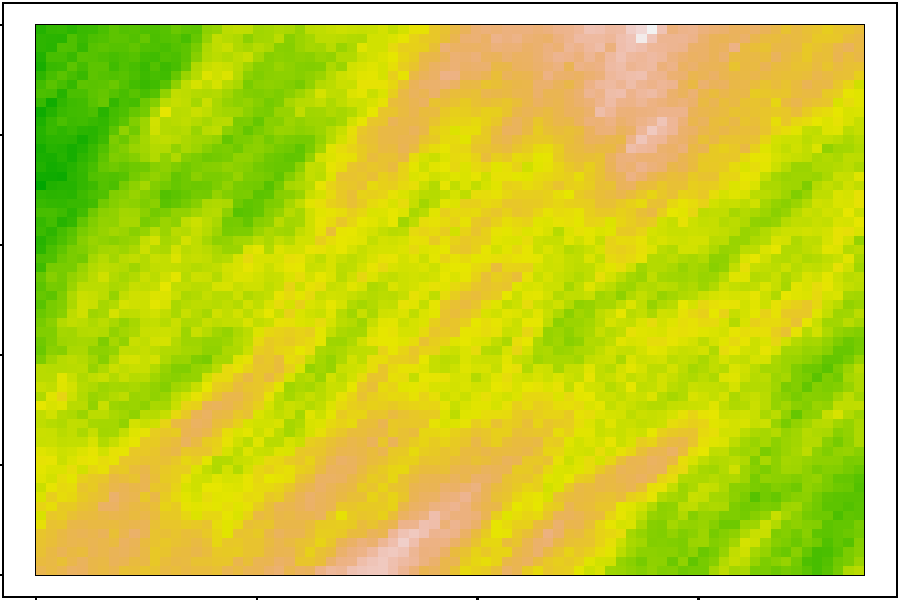
\includegraphics[width=0.45\textwidth]{figure/maternplot-3} 
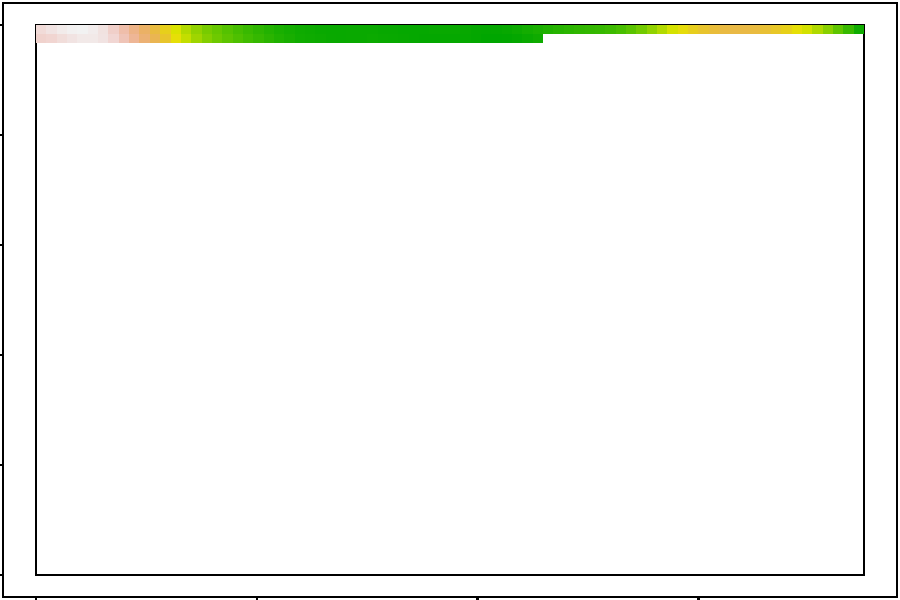
\includegraphics[width=0.45\textwidth]{figure/maternplot-4} 
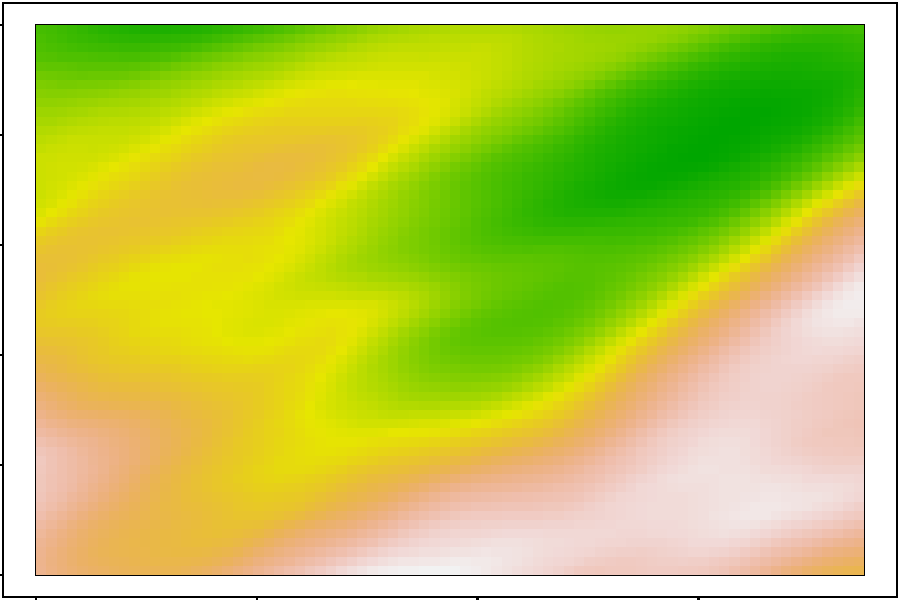
\includegraphics[width=0.45\textwidth]{figure/maternplot-5} 
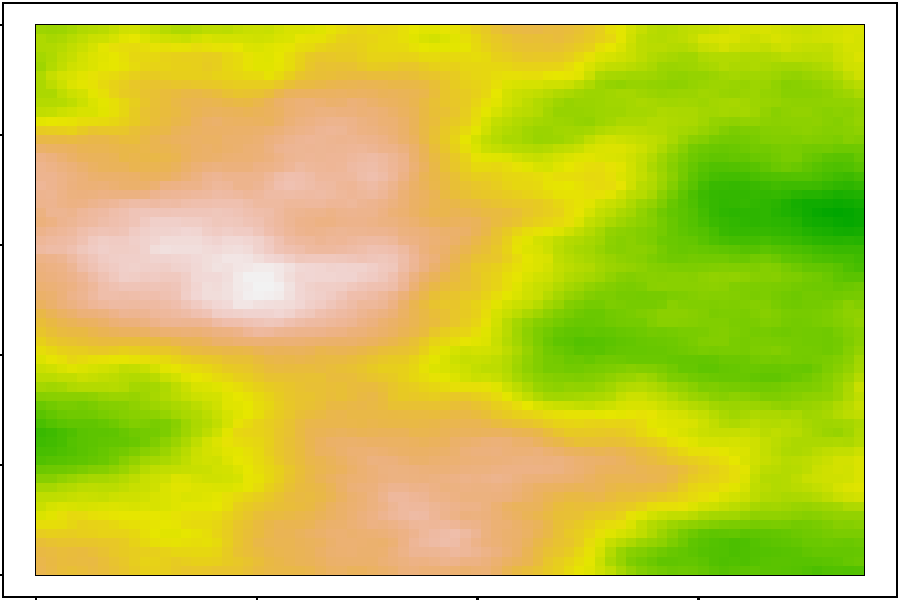
\includegraphics[width=0.45\textwidth]{figure/maternplot-6} 
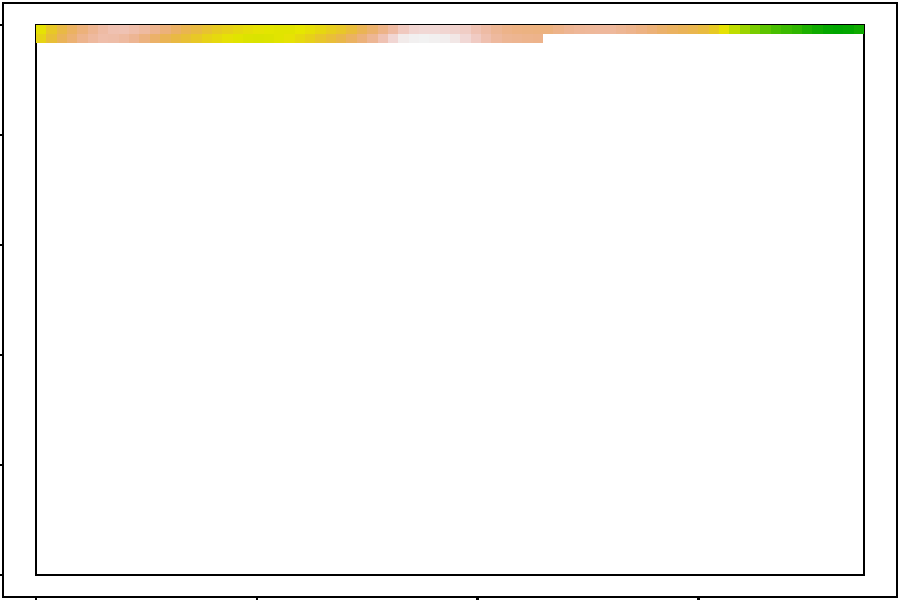
\includegraphics[width=0.45\textwidth]{figure/maternplot-7} 
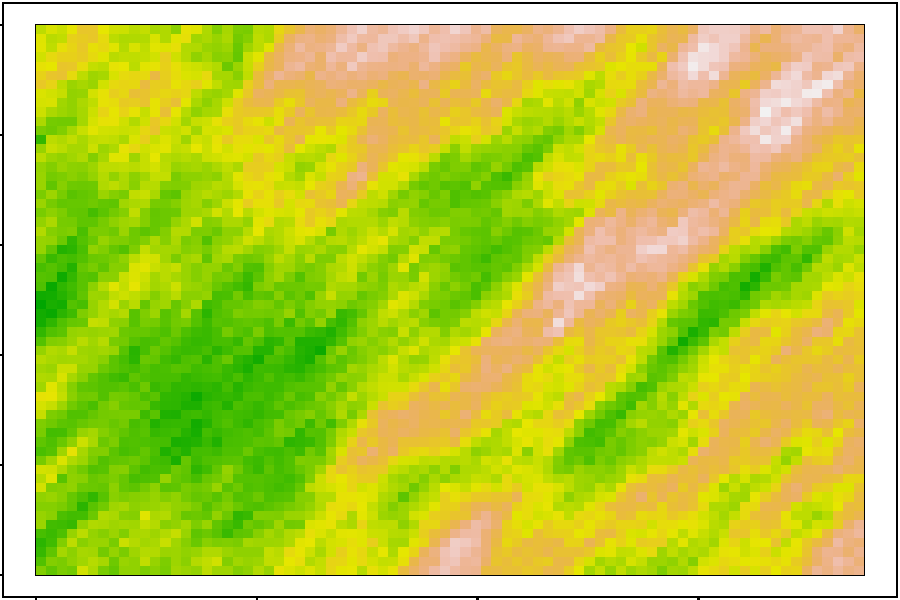
\includegraphics[width=0.45\textwidth]{figure/maternplot-8} 
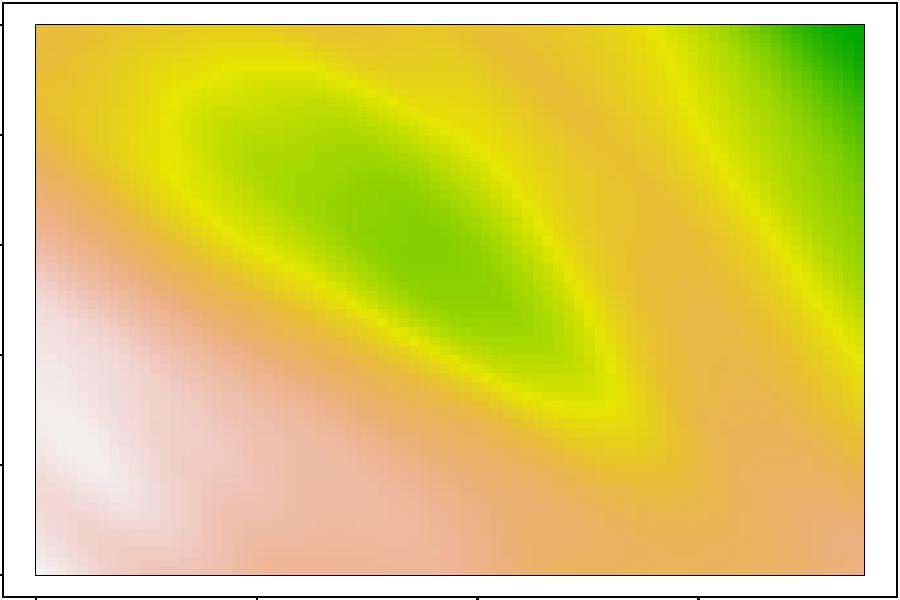
\includegraphics[width=0.45\textwidth]{figure/maternplot-9} 
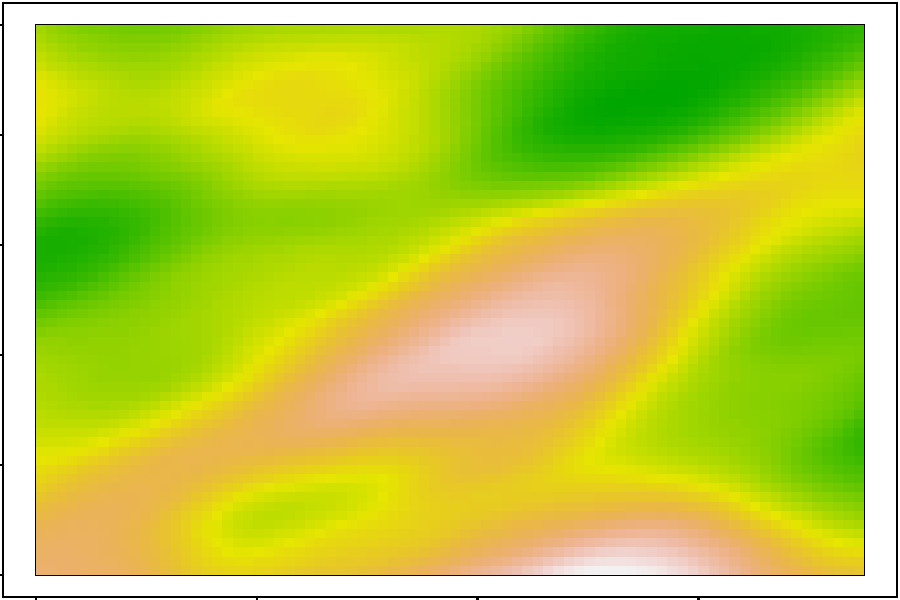
\includegraphics[width=0.45\textwidth]{figure/maternplot-10} 
\end{knitrout}
\caption{\label{fig:5} }
\end{figure}










\section{Discussion}
The package \pkg{gpuRandom} has been created to make GPU-generated uniform and normal random numbers accessible for \proglang{R} users, it enables reproducible research in simulations by setting seeds in streams on GPU. We further applied the GPU-generated random numbers in suitable statistical simulations, such as the Monte Carlo simulation for Fisher’s exact test, and (exact) Gaussian spatial surfaces simulation, for which we are able to calculate quantiles for the Normal distribution, compute mat\'ern covariance matrices, do Cholesky decomposition and matrix multiplication in batches on GPU. Most of these functions uses local memory on GPU, all of them uses parallel programming and avoids unnecessary data transfers between host and device. Comparison of performance between using \pkg{gpuRandom} and using classic \proglang{R} on CPU for some real data examples has demonstrated significant improvement in execution time. 

By leveraging the \pkg{gpuR} package, \pkg{gpuRandom} provides a user-friendly interface that bridges \proglang{R} and \proglang{OpenCL}, users can use the facilities in our package without the need to know the complex \proglang{OpenCL} or even the \proglang{\texttt{C++}} code.  \pkg{gpuRandom} is portable as its backend \proglang{OpenCL} supports multiple types of processors, and it is also flexible as its kernels can be incorporated or reconstructed in other \proglang{R} packages for further development. 

One of the main difficulties in developing the package is bug fixes and uncertain software behaviors. Error messages are often vague and it is time-consuming to locate the error within the backend \proglang{C} program. The usual steps that we take to debug is commenting out some parts of codes and then recompile many times until we find the problem, or printing out flag messages in several places in the code to find out where the program stops at due to error. \pkg{gpuRandom} is limited by the number and type of \proglang{OpenCL} RNGs used and the features of the \pkg{gpuR} package, as it depends upon the \pkg{gpuR} package, if developers wants to use our package to do something that's not supported in \pkg{gpuR}, for example ``sparse'' class objects, they would have to write \proglang{OpenCL} code to implement it.

Future work on \pkg{gpuRandom} package could be: (1) Explore other RNGs, for example the MRG32k3a, LFSR113, and Philox-4×32-10 generators in \proglang{clRNG} library, and compare the \proglang{R} performance between using different GPU RNGs. (2) Now that the package can do Cholesky decomposition and matrix multiplication in batches on GPU, which is a motivation for us to work on parallel likelihood evaluations on GPU for Gaussian spatial models in the next step. (3) Create a ``sparse'' matrix class on GPU and use it for simulating Gaussian random fields with sparse correlation structures such as the Gaussian Markov random fields.





\bibliography{paper1}




\newpage

\begin{appendix}


\end{appendix}


\end{document}

